% -*-cap2.tex-*-
% Este fichero es parte de la plantilla LaTeX para
% la realización de Proyectos Final de Carrera, protegido
% bajo los términos de la licencia GFDL.
% Para más información, la licencia completa viene incluida en el
% fichero fdl-1.3.tex

% Copyright (C) 2009 Pablo Recio Quijano 

% MANUAL DE USUARIO

% FIXME
% subir al apartado de ficheros de RedIRIS los manuales

\section{Ejecución}

En este capítulo veremos el funcionamiento de la aplicación desde el punto de vista de un usuario final que ejecutará el
videojuego con la intención de disfrutar de las opciones que ofrece. \\

Si el programa está instalado, se ejecuta con:

\begin{lstlisting} [language=Bash, numbers=left]
user@machine:~$ python dominous.py
\end{lstlisting}

o con un simple doble click si nos encontramos en un entorno windows. \\

\section{Menú principal}

El menú principal ofrece las siguientes opciones:

\begin{figure}[h]
  \label{screenshots_menu}
  \begin{center}
    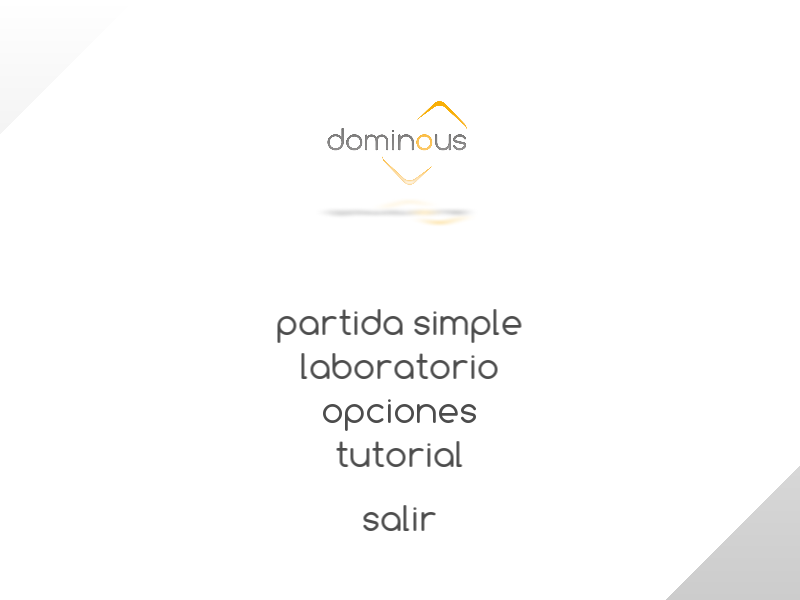
\includegraphics[scale=0.8]{screenshots_menu.png}
  \end{center}
  \caption{Menú principal de Dominous}
\end{figure}

\begin{description}
    \item[Partida simple] Será la poción más utilizada, ya que permite al usuario disfrutar de una partida de dominó.
    \item[Laboratorio] El modo laboratorio enfrenta a dos equipos controlados por el ordenador a cien partidas, para
            intentar dilucidar qué equipo es mejor.
    \item[Opciones] Las opciones del juego nos permite configurar la partida a nuestras necesidades, como veremos en el
            siguiente apartado.
    \item[Tutorial] Nos muestra un conjunto de diapositivas o transparencias con información rápida sobre cómo jugar,
            qué nos ofrece Dominous y unas breves nociones de juego del dominó.
    \item[Salir] Cierra y sale del juego.
\end{description}

Para movernos entre las distintas opciones simplemente debemos utilizar el ratón e ir clicando en las diferentes secciones,
pulsando el botón volver para retornar al menú principal en cualquier momento. Continuemos el manual mostrando la sección
tutorial y viendo las opciones que nos ofrece.

\section{Opciones}

Las opciones de juego, tal y como hemos comentado previamente, nos permite adaptar diferentes opciones de Dominous según
nuestras necesidades. Las opciones que se muestran son las siguientes:

\begin{figure}[h]
  \label{screenshots_options}
  \begin{center}
    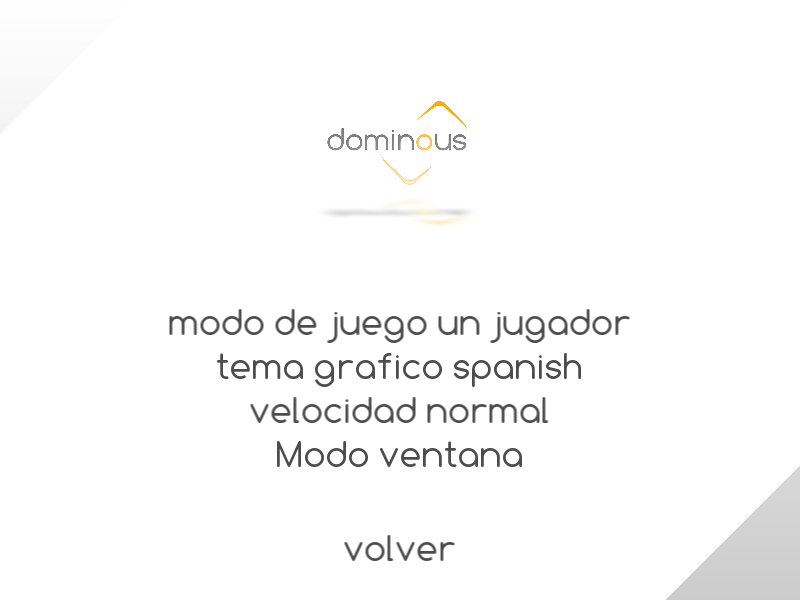
\includegraphics[scale=0.8]{screenshots_options.png}
  \end{center}
  \caption{Pantalla de opciones de juego}
\end{figure}

\begin{description}
    \item[Modo de juego] Podemos seleccionar si, en el modo de juego \textbf{partida simple}, queremos participar nosotros
        como jugador activo o simplemente queremos observar cómo el ordenador desarrolla la partida completa, controlando
        él mismo a todos los jugadores. 
    \item[Tema gráfico] Esta opción nos permite seleccionar el aspecto gráfico de la partida. El aspecto gráfico permite
        cambiar la visualización de fichas, mesa de juego y otros elementos, al estilo de los temas gráficos que poseen
        los sistemas operativos.
    \item[Velocidad de juego] Dominous posee tres tipos de velocidades de juego:
        \begin{itemize}
            \item Velocidad normal --- el juego se desarrolla a una velocidad pausada, con movimientos de fichas que permiten
                seguir el transcurso de la partida con comodidad, y se muestra información sobre el tiempo que emplea cada
                jugador mientras piensa la jugada a ejecutar.
            \item Velocidad rápida --- las fichas se mueven a la misma velocidad que en el modo normal, pero los jugadores
                colocan la ficha inmediatamente en cuanto les toca su turno.
            \item Velocidad extra rápida --- el movimiento de las fichas es acelerado y los jugadores no emplean tiempo
                pensando la jugada
        \end{itemize}
    \item[Modo ventana] Lorem ipsum dolor
\end{description}

\begin{figure}[h]
  \label{screenshots_themes}
  \begin{center}
    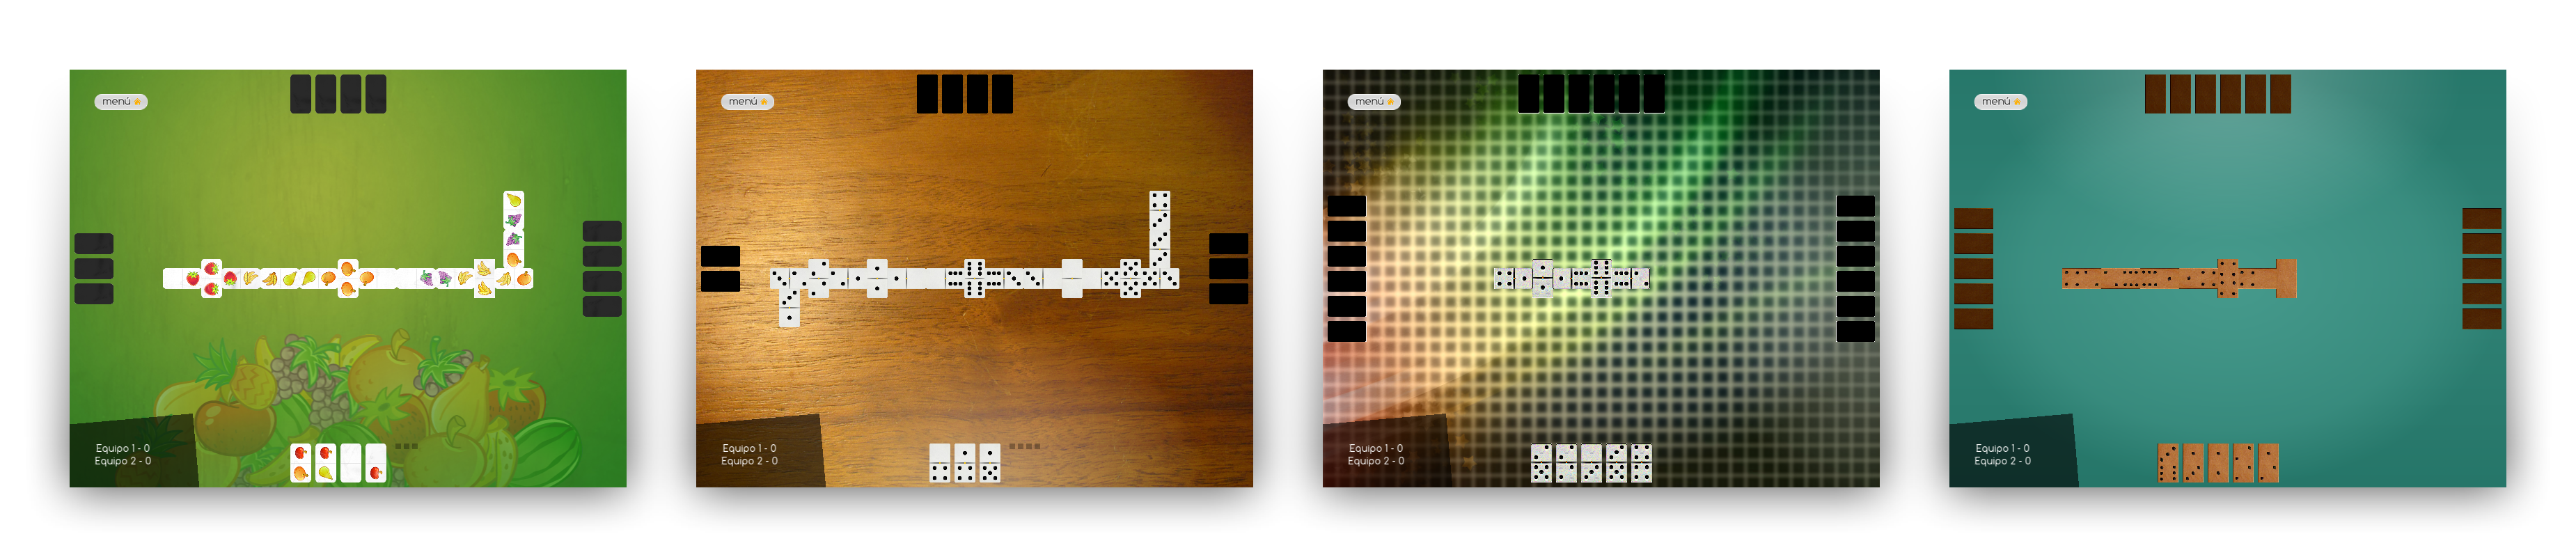
\includegraphics[scale=0.2]{screenshots_themes.png}
  \end{center}
  \caption{Diferentes temas gráficos que vienen de serie con Dominous}
\end{figure}

\section{Tutorial}

El tutorial de juego sirve de ayuda a los nuevos jugadores de Dominous, presentando de forma resumida todas las opciones
que posee Dominous y evitando que, en un primer uso, sea necesario leer todo el manual de usuario.

\begin{figure}[h]
  \label{screenshots_tutorial}
  \begin{center}
    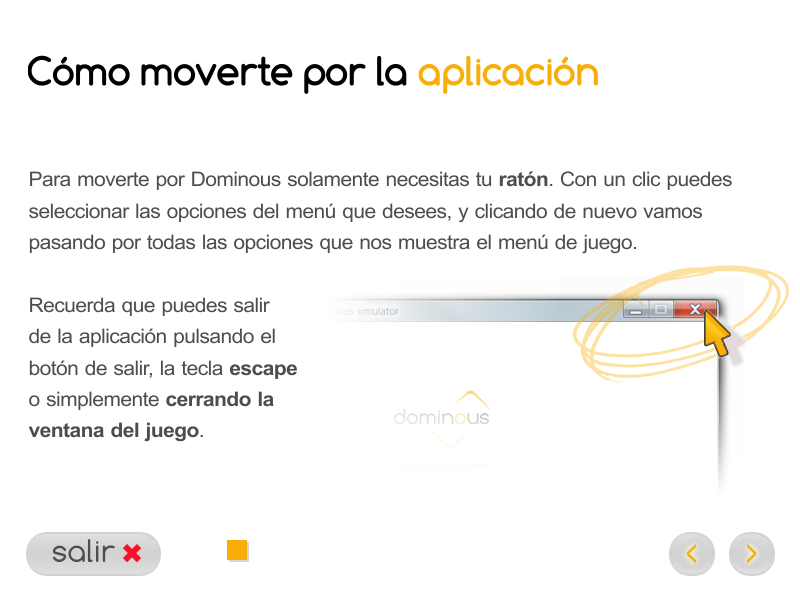
\includegraphics[scale=0.8]{screenshots_tutorial.png}
  \end{center}
  \caption{Modo tutorial, con instrucciones básicas de juego}
\end{figure}

\begin{itemize}
    \item Las primeras capturas informan sobre la interfaz de Dominous: cómo moverte por las opciones, salir del juego, jugar
        una partida, colocar fichas, entrar y salir de una partida de dominó, y diferentes elementos que se muestran a la
        hora de disfrutar de una partida.
    \item Luego se nos informa del modo Laboratorio, describiendo cada uno de los elementos que aparecen en pantalla como
        son las barras de información o la gráfica de partidas ganadas.
    \item Por último se pretende dar al usuario novel de unas nociones básicas de dominó: cómo jugar, cuántas fichas existen,
        breve explicación sobre el modo de juego por parejas y cierres.
\end{itemize}


